% Contributors: Luis Lopez, Robby Costales, Daniel Jaroslawicz, Colin Brown
\section{Problems with Training GANs}


GANs are notoriously difficult to train. Part of this difficulty stems from the fact that training is a dynamic process where both networks constantly update their parameters. Therefore, training is not a simple optimization problem, but instead an effort to find an equilibrium where neither the generator network nor the discriminator network can (significantly) improve performance by updating their parameters.

However, Arora et al. \cite{arora2017eq} prove that for certain natural training objectives (e.g. Wasserstein) there exists a pure approximate equilibrium in which the generator wins the game. Thus, the issue is not that no equilibrium where the generator fools the discriminator exists, but that a simple algorithm such as backpropagation does not necessarily find this equilibrium.

The idea behind the proof offered in \cite{arora2017eq} is that if we allowed our generator to be an infinite mixture of deep nets and assume that each deep net is capable of generating a simple Gaussian distribution, then the resulting distribution $\mathcal{D}_G$ is an infinite mixture of Gaussians. Since we know that an infinite mixture of Gaussians can closely approximate any distribution, such a generator can produce $\mathcal{D}_G$ matching $\mathcal{D}_{real}$ and therefore find an equilibrium where it wins. Similarly, if we only allow a finite mixture of deep nets then our generator can learn distribution $\mathcal{D}_G$ that the discriminator can only distinguish from $\mathcal{D}_{real}$ with probability $\leq \epsilon$.

More formally: for a class of generators $\{G_u, u \in \mathcal{U}\}$ and a class of discriminators $\{D_v, v \in \mathcal{V}\}$ we can define the payoff $F(u,v)$ of the game between the generator and discriminator
$$
F(u,v) = \E_{x \sim \mathcal{D}_{real}}[\phi{(D_v(x))}] + \E_{x \sim \mathcal{D}_G} [\phi(1 - D_v(x))].
$$

Where $\phi$ is some concave function (the logarithmic function in the original GAN paper). Additionally, define a pair of strategies for the discriminator and generator $(\mathcal{S}_u, \mathcal{S}_v)$ to be an $\epsilon$-approximate equilibrium if for some value $V$:
$$
\forall v \in \mathcal{V}, \:\:\: \E_{u \sim \mathcal{S}_u}[F(u,v)] \leq V + \epsilon;
$$
$$
\forall u \in \mathcal{U}, \:\:\: \E_{v \sim \mathcal{S}_v}[F(u,v)] \geq V - \epsilon.
$$

In words, this means that given a generator chosen according to the generator strategy, no matter what discriminator the discriminator strategy decides to use it cannot achieve expected payoff $> V + \epsilon$, and, similarly, given a discriminator chosen according to the discriminator strategy, no matter what generator the generator strategy decides to use it cannot achieve expected payoff $< V - \epsilon$. I.e. unilaterally altering the generator or discriminator can only allow a competitor to achieve a trivial performance gain. If the strategies $(\mathcal{S}_u, \mathcal{S}_v)$ are pure strategies then we call this an $\epsilon$-approximate pure equilibrium.

Now we can formalize our above claim that a generator consisting of a finite mixture of deep nets can learn distribution $\mathcal{D}_G$ that the discriminator can only distinguish from $\mathcal{D}_{real}$ with probability $\leq \epsilon$. Suppose that $\phi$ is $L_\phi$-Lipschitz and bounded in $[-\Delta, \Delta]$ and the generators and discriminators are $L$-Lipschitz with respect to the parameters and $L'$-Lipschitz with respect to inputs, and the generator networks all have $p$ parameters then:

\begin{theorem}
If the generator can approximate any point mass (for all points $x$ and any $\epsilon > 0$, there is a generator that in expectation over its input noise outputs a value within $\epsilon$ of $x$) there is a universal constant $C > 0$ such that for any $\epsilon > 0$, there exists $T = \frac{C\Delta^2 p \log(p L L' L_\phi / \epsilon)}{\epsilon^2}$ generators $G_{u_1}, \cdots G_{u_T}$. Let $\mathcal{S}_u$ be a uniform distribution on each $u_i$, and $D$ be a discriminator that outputs only $\frac{1}{2}$, then ($\mathcal{S}_u, D$) is an $\epsilon$-approximate equilibrium.
\label{thm:gen}
\end{theorem}

The idea of the proof of the theorem is that since the generator can approximate any point mass, an infinite mixture of generators can approximate the target distribution $\mathcal{D}_{real}$. Then, using a probabilistic argument and epsilon net argument to show that if we sample $T$ generators and discriminators from an infinite mixture, they form an approximate equilibrium with high probability. So we see that a mixture of $O(p)$ generators can achieve an $\epsilon$-approximate equilibrium in which they win.

We can use this result to show that if we have deep nets of size $p$ that are capable of approximating any point mass then we can build a generator of size $O(p^2)$ that has an approximate equilibrium in which it wins. The idea is that given a mixture of $T$ generator nets with $k$ layers and $p$ parameters we can combine them all into a single $k+1$-layer network with $O(p^2)$ parameters that approximately generates the same distribution as the mixture of nets. Simply run the input $h$ through all $T$ networks and then add on a "selector" layer that selects the output of one of the networks with appropriate probability.

The authors use this theoretical result to suggest a practical improvement to GAN architecture called the MIX+GAN that can potentially improve the stability of training. Essentially, instead of training a single discriminator and generator, an ensemble of generators and discriminators are trained together along with the probability weights assigned to each generator. A regularizing term is added to keep the weights close to uniform so that all generators in the mixture are used to some degree. On some empirical experiments such an architecture offers some Inception Score improvement.

\subsection{Generalization of the Learned Distribution}
Aside from difficulties in the training process, the distribution learned by the generator network can have various issues as well.

\subsubsection{Distance of the Learned Distribution from the Target Distribution}

Arora et al. \cite{arora2017eq} demonstrate that for typical notions of distance between distributions (e.g. Wasserstein, Jensen-Shannon), and a polynomial number of samples from the target distribution $\mathcal{D}_{real}$ available, generalization is not guaranteed. The generator can win even when $\mathcal{D_G}$ and $\mathcal{D}_{real}$ are arbitrarily far in any of the standard metrics, where $\mathcal{D_G}$ is the learned distribution of the generator.

Formally, we can define GAN generalization in a similar way to generalization error in a supervised learning context. Given $\hat{\mathcal{D}}_{real}$, an empirical version of the target distribution with $m$ samples, a generated distribution $\mathcal{D}_G$ generalizes under the distance between distributions $d(\cdot, \cdot)$ with generalization error $\epsilon$ if, with high probability:
$$
|d(\mathcal{D}_{real}, \mathcal{D}_G) - d(\hat{\mathcal{D}}_{real}, \hat{\mathcal{D}}_G)| \leq \epsilon
$$

Where the second term deals with the empirical distributions over a polynomial number of samples (otherwise our training algorithm cannot run in a reasonable amount of time).

To see that JS divergence and Wasserstein distance don't generalize with a polynomial number of examples under this definition, consider target distributions $\mu$ that are uniform Gaussian distributions $\mathcal{N}(0, \frac{1}{d}I)$ and let $\hat{\mu}$ be empirical versions of $\mu$ with $m$ examples. In this case we have $d_{JS}(\mu, \hat{\mu}) = log2$ and $d_{W}(\mu, \hat{\mu}) \geq 1.1$.

Now, if $\mathcal{D}_{real} = \mathcal{D}_G = \mu$ then we have $d_{W}(\mathcal{D}_{real}, \mathcal{D}_G) = 0$ but $d_{W}(\hat{\mathcal{D}}_{real}, \hat{\mathcal{D}}_G)) > 1$ as long as we only have a polynomial number of examples. A similar argument goes for the case where $\hat{\mathcal{D}}_{real} = \mathcal{D}_G = \hat{\mu}$ and for the JS divergence.

The authors go on to show that the distance metric GANs actually minimize is what they refer to as the \emph{neural net distance}. In particular, let $F$ be a class of functions from $\bbR^d$ to $[0,1]$, then define the \emph{F-divergence} with respect to measuring function $\phi$ between two distributions $u, v$ as:
$$
d_{F, \phi}(u,v) = sup_{D \in F} \E_{x \sim u}[\phi(D(x))] - \E_{x \sim v}[\phi(1 - D(x))] - 2\phi(\frac{1}{2})
$$

This should look familiar to us. Suppose $F$ is a set of neural networks and $\phi(t) = log(t)$, then the GAN objective function we defined in section 3.1 is equivalent to $min_G d_F(\hat{\mathcal{D}}_{real}, \hat{\mathcal{D}}_G)$. We call $d_F$ where $F$ is a set of neural nets with a bound $p$ on the number of parameters the neural net distance. Under the neural net distance, GANs do generalize. Formally:

\begin{theorem}
Let $u, v$ be two distributions and $\hat{u}, \hat{v}$ be empirical versions of these distributions with at least $m$ samples each. There is a universal constant $C > 0$ such that when $m \geq \frac{c\Delta^2 p \log(p L L_\phi / \epsilon)}{\epsilon^2}$ we have with probability at least 1 - exp(-p) over the randomness of $\hat{u}, \hat{v}$ that:
$$
|d_{F, \phi}(u,v) - d_{F, \phi}(\hat{u}, \hat{v})| \leq \epsilon
$$
\label{thm:gen}
\end{theorem}

Where $L, and L_\phi$ are defined similarly as in section 4.1. The intuition is that there aren't too many distinct discriminators, and thus given enough samples we can use concentration bounds to show that the expectation over the empirical distribution converges to the expectation over the true distribution for all discriminators.

However, this weaker metric may be near zero (implying good generalization) even when the learned distribution and the target distribution are very far. This is because the a discriminator limited to size $p$ cannot distinguish between a target distribution $\mu$ and a distribution with a low support of only $O(\frac{p}{\epsilon^2})$.

\subsubsection{Low Support of the Learned Distribution}

In the paper \textit{Do GANs Learn the Distribution? Some Theory and Empirics} \cite{arora2018do}, Arora et al. raise further questions on the on the robustness of GANs. They first present a new test based on the \textit{birthday paradox} designed to estimate the support size of the learned distribution of the generator. Upon evaluation on multiple models and datasets, results show that even certain state-of-the-art the GANs learn distributions of low support. The authors then devise a theoretical failure case for encoder-decoder GANs specifically, showing these architectures are still susceptible to mode collapse, and are even capable of learning entirely meaningless representations while achieving a low objective. Both contributions highlight significant issues with the current state of GANs.

% - birthday paradox test formulation

The birthday paradox refers to the seemingly unlikely result that even in relatively small groups of people, it is likely that at least one pair share the same birthday. More formally, it says that in a population distribution with support \textit{N} (\textit{support} being the number of points with nontrivial probability mass), batches of size $\sqrt{N}$ are likely to have a duplicate. The authors use this fact as a key insight in the design of their test. If a batch containing \textit{s} GAN-generated images contains a duplicate slightly more often than not, one can estimate the support of the learned distribution to be around $s^2$. Since GANs generate continuous outputs, the authors flag the top 20 (arbitrary choice) most similar images using a computed metric, and then manually identify duplicates among this set by sight. This manual checking is seen as necessary since even the most commonly used metrics for GANs are flawed \cite{barratt2018note}, and the goal after all is to generated images that satisfy human judgement.

% - birthday paradox results (include figures from paper)

\begin{figure}[t]
    \centering
    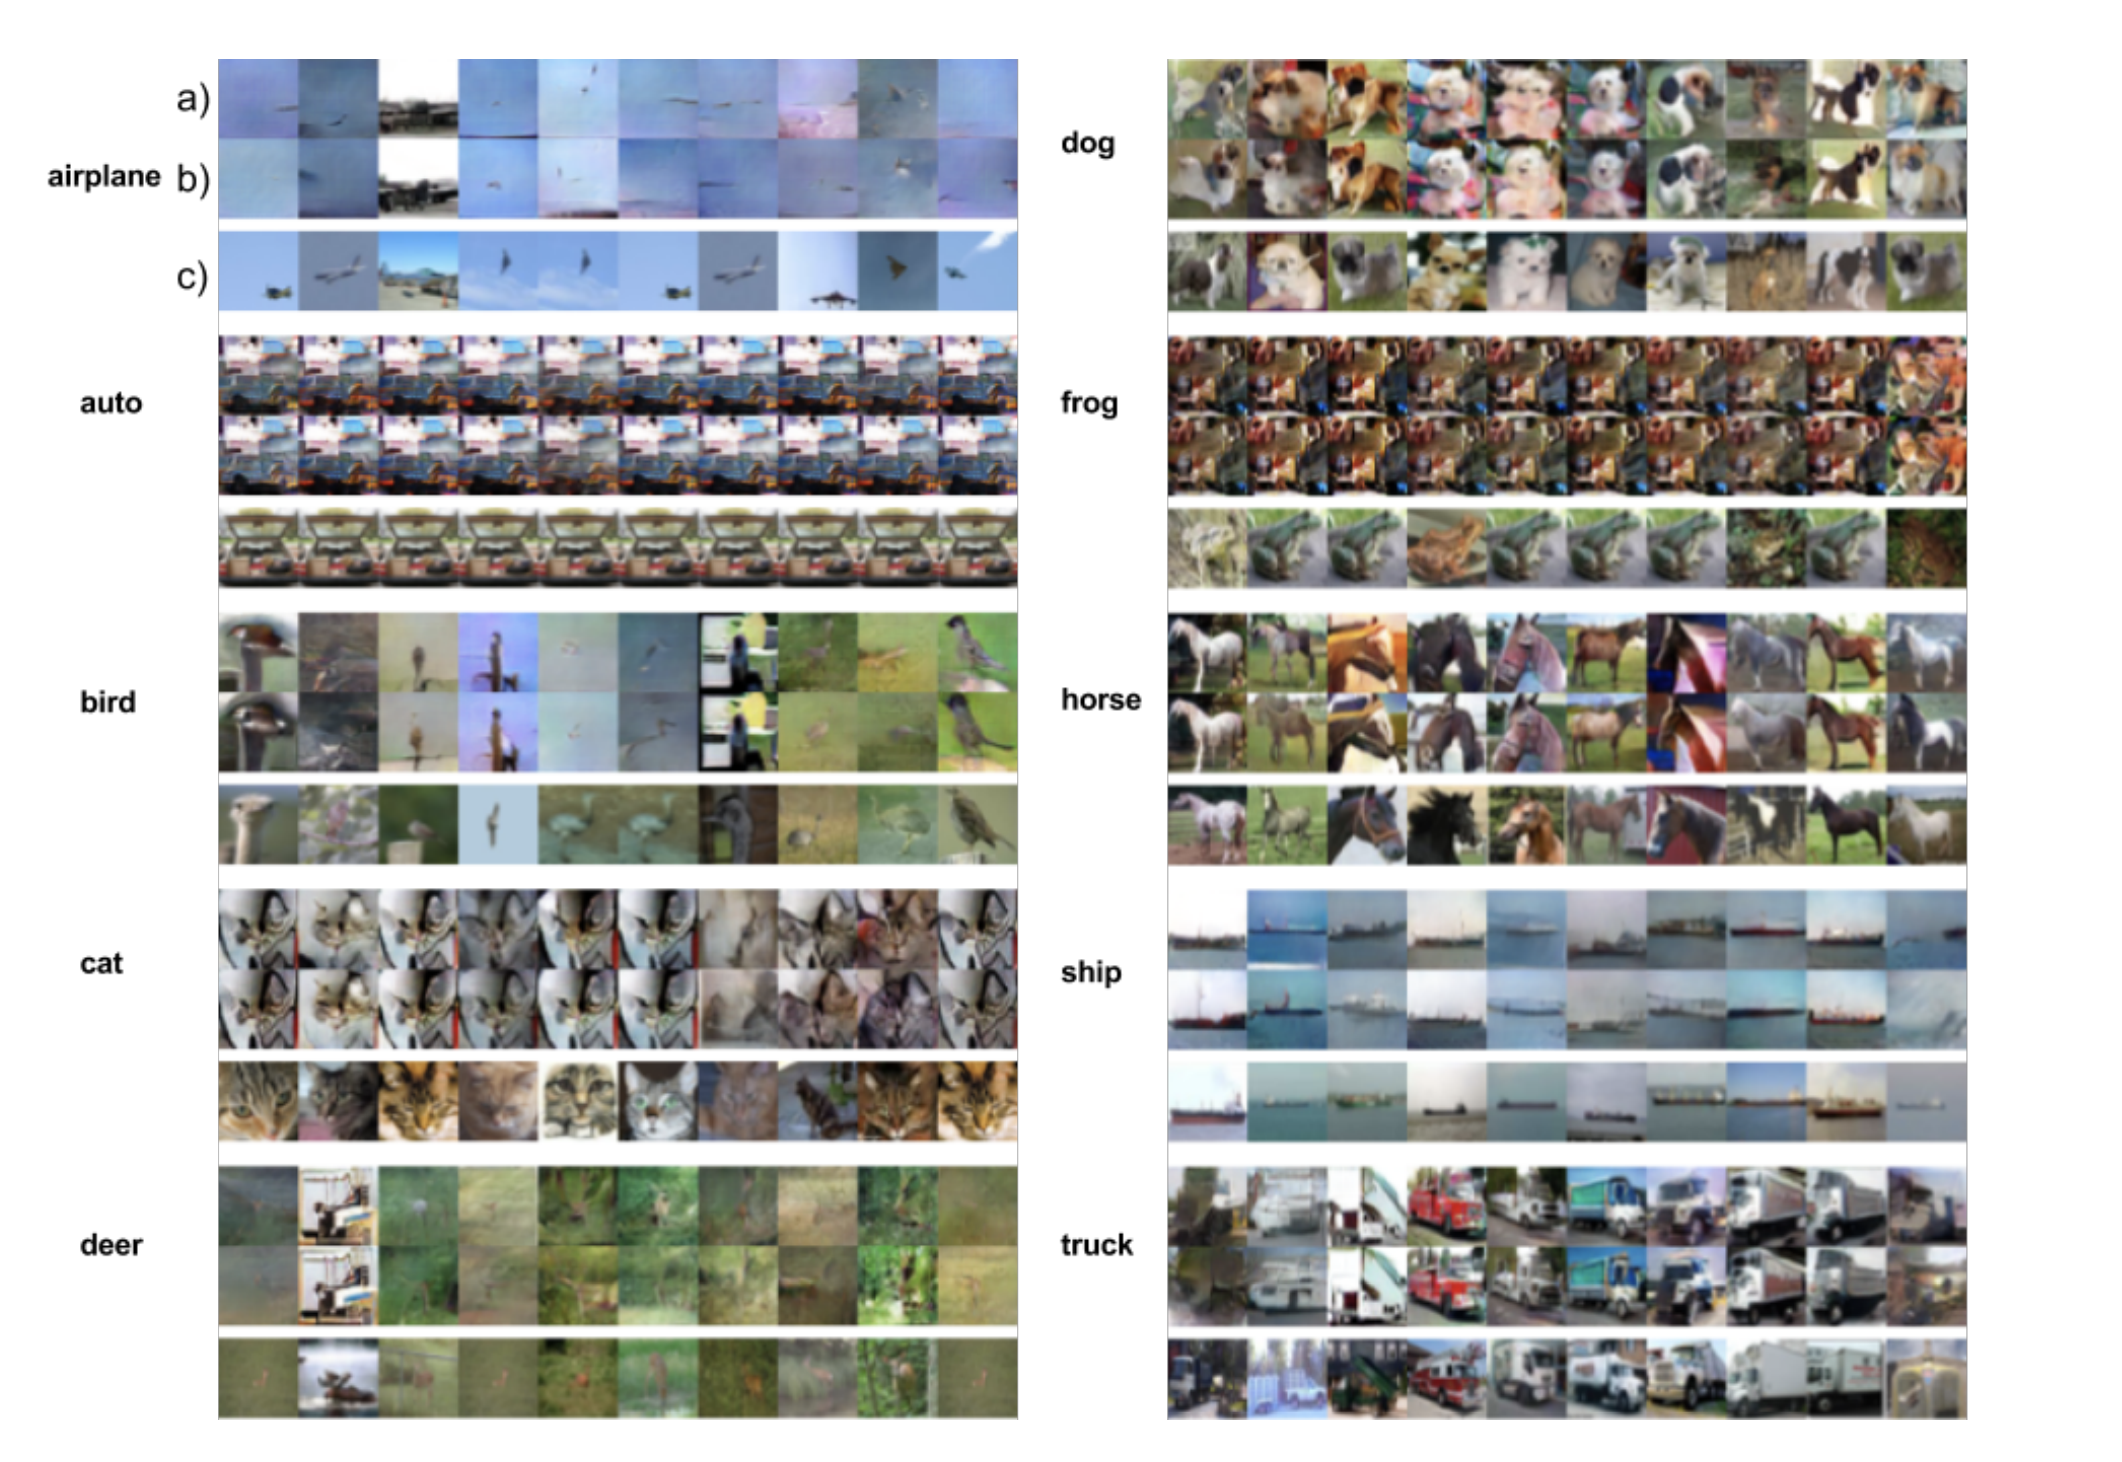
\includegraphics[width=1.0\linewidth]{chapter_14/files/cifar10dup.png}
    \caption{``Duplicate pairs found in a batch of 1000 generated CIFAR-10 samples from a Stacked GAN.a)-b):pairs of duplicate samples; c): nearest neighbor of b) in the training set." \cite{arora2018do}}
    \label{fig:cifar10dup}
\end{figure}

The authors use this technique to evaluate multiple GAN models trained on CIFAR-10 and CelebA, two popular computer vision datasets. They find that for both DCGAN \cite{goodfellow2014generative, radford2015unsupervised} and MIX+DCGAN \cite{Ma_2018} models, a batch size of around 800 is sufficiently large to produce duplicates with probability $\geq 50\%$. This implies that the support of learned distribution is less than 640,000 ($800^2$), which is on the same order of the size of the training set. However, from the dissimilarity between samples in the generated set and their nearest neighbors in the training set, we can see that the samples were not memorized at least. For ALI \cite{dumoulin2016adversarially} and BiGANs \cite{donahue2016adversarial}, the estimated support is six times larger than the training set, supporting claims from \cite{dumoulin2016adversarially, donahue2016adversarial} that ``the bidirectional structure prevents some of the mode collapse observed in usual GANs" \cite{arora2018do}. For CIFAR-10, the authors estimated support separately for each of the 10 classes; the values ranged from $50^2$ to $500^2$ among the various classes. Again, the closest images appear not to be duplicates, so the generator is not simply memorizing the training set. See \ref{fig:cifar10dup} for examples of duplicates found in each class.

% - "limitations of encoder-decoder GAN architectures" proof sketch and implications

Next, the authors of \cite{arora2018do} narrow their scope to encoder-decoder GAN architectures \cite{dumoulin2016adversarially, donahue2016adversarial}---the same ones that were found to learn distributions of higher support in the previous results---and show that they have the same problem of mode-collapse as other GAN architectures, and specifically prove the existence of a setup in which the encoder learns practically meaningless information. The authors provide a proof sketch of this result in the paper; the full proof exists in the appendix due to its length and technical involvement. We will share the main theoretical result here, and provide some intuition for it. The main theorem is as follows, taken directly from \cite{arora2018do}.

\begin{theorem}
There exists a generator G of support $\frac{p\Delta^2 \log ^2 (p \Delta L L_\phi / \epsilon)}{\epsilon^2}$ and an encoder E with at most $\tilde{d}$ non-zero weights, s.t. for all discriminators D that are L-Lipschitz and have capacity less than p, it holds that

$$
| \E_{x \sim \mu} \phi ( D (x, E(x))) - \E_{z \sim \nu} \phi (D(G(z), z)) | \leq \epsilon
$$
\label{thm:gen}
\end{theorem}

The idea is that an encoder of small complexity and a generator of small support are able to produce a small (satisfactory) BiGAN training objective. The authors define the meaningless information that is to be extracted from the inputs as sparsely placed noise, which is a function of the variables in the latent space (i.e. the random code used as input for the generator). We can can define the encoder as a function that simply extracts this noise, thereby retrieving the necessary information about the latent space directly. This encoder can be trivially constructed using a ReLU network that links to the necessary pixels (hence the ``$\tilde{d}$ nonzero weights"). The generator is designed to learn a distribution support of $m := \frac{p\Delta^2 \log ^2 (p \Delta L L_\phi / \epsilon)}{\epsilon^2}$. The proof of Theorem \ref{thm:gen} is accomplished by defining a distribution over a specific set of generators, and showing with high probability one of the generators in the set satisfies the theorem statement \cite{arora2018do}. This result suggests that we may not simply be able to ``let BiGANs be BiGANs".
